\section{Project organization and means implemented}
\label{sec:org}

\subsection{Scientific coordinator and its team}

\Comments{
  In the case of a Young Researchers Project (JCJC), 
Present the scientific coordinator and his/her role in the project, present his/her position within the organization of the host laboratory 
Present the scientific coordinator’s team, its quality and complementarity
}

%------------------------ team
\textbf{Tristan Roussillon} (33 years old) is the principal investigator (PI) of the project
and will be involved in all the tasks. Implication: \textbf{30} person months (PM). 
He completed his PhD in 2009 and since 2012, he is an associate professor in Computer Science at INSA Lyon
and a member of LIRIS. 
He has coauthored a book chapter on digital geometric estimators \cite{Coeurjolly2012} and
has recently obtained several results on normal vector computation \cite{LPRTCS2016,LPRDGCI2016,LPRJMIV2017}.    
He has coauthored several papers in peer-reviewed international journals (\eg PR, CVIU, JMIV, DAM) 
and in conferences (\eg DGCI, ICPR).

The project will also involve specialists in digital geometry and combinatorics on words.
%(see also table~\ref{tab:persons}). 
\begin{table}[h]
\small
\centering
\begin{tabular}{|ccclr|}
\hline
Collaborator & Position & Lab & Expertise & PM\\ \hline
\hline
\textbf{D. Coeurjolly} & DR & LIRIS & digital and comput. geometry, geometry processing & 5 \\ \hline
\textbf{B. Kerautret} & MdC & LORIA & digital geometry, image analysis & 12 \\ \hline
\textbf{S. Labb\'{e}} & CR & LABRI & multidim. cont. frac. alg., combinatorics on words & 12 \\ \hline
\textbf{J-O. Lachaud} & Pr & LAMA & digital geometry and topology, image analysis & 6 \\ \hline
\hline
\end{tabular}
\normalsize
\end{table}
%% \begin{table}[h]
%% \small
%% \centering
%% \begin{tabular}{|ccclcc|}
%% \hline
%% Collaborator & Position & Lab & Expertise & WP & PM \\ \hline
%% \hline
%% \textbf{D. Coeurjolly} & DR & LIRIS & digital and comput. geometry, geometry processing & 2-3 & 5 \\ \hline
%% \textbf{B. Kerautret} & MdC & LORIA & digital geometry, image analysis & 3 & 12 \\ \hline
%% \textbf{S. Labb\'{e}} & CR & LABRI & multidim. cont. frac. alg., combinatorics on words & 0-1 & 12 \\ \hline
%% \textbf{J-O. Lachaud} & Pr & LAMA & digital geometry and topology, image analysis & 0,2-3 & 6 \\ \hline
%% \hline
%% \end{tabular}
%% \normalsize
%% \end{table}


\textbf{D. Coeurjolly} (40 years old) is a senior tenured
  researcher (\emph{Directeur de recherche}) at CNRS and a member of
  LIRIS since 2007. His research interests include digital and
  computational geometry, geometry processing and sampling in computer
  graphics. From 2006 to 2008, he chaired the Technical Committee 18
  "Discrete Geometry" of IAPR (Int. Assoc. for Pattern
  Recognition). In 2008, he chaired and organized the International
  conference on Discrete Geometry for Computer Imagery (DGCI 2008) in
  Lyon. Since 2011, he chairs the Steering Committee of the DGCI
  conference. 
  %From 2011 to Jan. 2015, he lead the \emph{m2disco} team at LIRIS and
  Since 2017, he is Director of the Fédération Informatique de Lyon
  (FR2000, CNRS).
  In 2009, he received a Bronze Medal from CNRS that
  recognized his activities in digital geometry. He has
  authored/co-authored 35 articles in the main international journals
  of the field (\eg TOG, PAMI, IP, CVIU, PR, PRL, DAM, GMOD, C \& G,
  IVC), and more than 40 papers in peer-reviewed international
  conferences (\eg SIGGRAPH, DGCI, ICPR, IWCIA).
  %%TRIS: 
  In 2010, he co-created {\DGtal} and he is now one of
  the main editor of the library.


  
 \textbf{B. Kerautret} (41 years old) is an assistant professor since 2005
 at the LORIA laboratory. He received a PhD degree in Computer
 Science from Bordeaux University in 2004.  His research are
 focused on digital geometry, image processing and its applications.
 He co-organized the International conference on Discrete
 Geometry for Computer Imagery (DGCI 2011) in Nancy. He
 is also interested in reproducible research as an active member of the
 IPOL Editorial Board and was at the initiative of the recent
 first workshop on Reproducible Research in Pattern Recognition in
 2016.
 %He participate to the GeoDIB ANR project in 2006-2011 and co advised 2 Phd Thesis.
 Since 2017, he chairs the Technical Committee 18 "Discrete Geometry" of IAPR
 (Int. Assoc. for Pattern Recognition). He has written
 about forty papers in international journals or conferences on these
 topics. He actively contribute to {\DGtal} library and is the manager of
 the {\DGtalTools} project.
 %part of DGtal dedicated to applications. %%TRIS deja presente (sec. 1)
 In december 2017, he defended his habilitation thesis to supervise research.
 %habilitation to conduct researches.
 

\textbf{S. Labb\'{e}} (34 years old) completed his PhD in Montreal in 2012, is
a CNRS researcher at LaBRI (Bordeaux) since 2017 after two two-years
postdoctorate in LIAFA (Paris, France) and Université de Liège (Liège,
Belgique).  He has a lot of experience with multidimensional continued
fractions (MCF) algorithms \cite{arnoux_labbe_2017,cassaigne_a_set_2017} in
relation to combinatorics and discrete geometry.  He is an active developper of
the Sage math software since 2008 and is developping an optional Sage package
containing currently 30k lines of documented code \cite{labbe_slabbe_0_4_2018}
on combinatorics, dynamical systems and discrete geometry allowing many kinds
of experimentations including the comparison of various MCF algorithms
\cite{labbe_3-dimensional_2015}.  His research on the generalization of
Christoffel words in arbitrary dimension \cite{Labbe2015} is fundamental for
the realization of the work package 1 of the current project.  He as coauthored
17 papers in peer-reviewed international journals (\eg JMAA, ETDS, DGC, TCS,
EJC, AAM, DAM, DMTCS) and 17 papers in conferences (\eg DGCI, WORDS, DLT).

\textbf{J-O. Lachaud}

%TODO research highlights en citant des contributions dans le domaine. 

This team gathers all the expertise required to ensure the success of the project.
Furthermore, this project will let the team members maintaining their lead in digital surface analysis 
and more generally in digital geometry and combinatorics on words for digital imagery. 


\subsection{Means of achieving the objectives}

%% In this section, we first detail and justify the scientific programme with regard to the project objectives.
%% We then describe the requested means. 

\subsubsection{Scientific programme}
\label{sec:wp}

\Comments{Set out the scientific programme and justify the work programme's task breakdown with regard to the objectives being pursued.
For each task, describe the objectives, the work programme, deliverables, partners' contributions, methods and technical decisions, risks, and fall-back solutions. 
Illustrate the programme with a Gantt chart. 
}

PARADIS aims at analyzing digital surfaces. Our approach will consist in finding
digital plane segments onto digital surfaces \ref{goalppa} and deriving first-order
estimates such as normal direction \ref{goalestim}. Digital plane segments will
also provide a way of detecting meaningful scales automatically \ref{goalscale}.

Toward these goals, we propose four work packages (WP) summarized below and
developed within this section. The first two are devoted to the improvement of
plane-probing algorithms, which will be our main tool to achieve goals \ref{goalestim}
and \ref{goalscale} in the last two packages. 

\begin{enumerate} [label=(W\arabic*),start=0]
\item Plane-probing algorithms (first year). In this WP, we will seek to
  improve various features of plane-probing algorithms, even in the
  planar case. Thanks to our preliminary works, we have in mind many short-term
  tasks for this.  \label{wp0}
\item Pattern generation (first two years). In this WP, we will seek a way to associate
  to the state of a plane-probing algorithm a piece of digital plane
  that fits the digital surface in order to correctly process non-planar parts,
  especially non-convex parts. This requires not only expertise in
  digital geometry but also in multidimensional continued fractions
  algorithms and combinatorics on words (see \sect{sec:dps} and below).  \label{wp1} 
\item Geometric inference and applications (years 2 and 3). This WP is devoted
  to the derivation of efficient, parameter-free, multigrid-convergent estimators.
  The goal of this WP is also to investigate at least one application based on
  first-order estimators, such as surface fairing. \label{wp2} 
\item Multiscale analysis of digital surface (years 3 and 4). In this WP, we will
  seek a way to locally detect the best scales of analysis, based on properties
  of digital plane segments. \label{wp3}
\end{enumerate}

Since there are so many perspectives and research directions, this project needs
to strengthen a team of experts by full-time workers in order to make the best of them.
We request a financial support for: 
\begin{itemize}
\item[(MS)] one master project funding to help us on short-term tasks in \ref{wp0},
\item[(PhD)] one PhD grant for working on \ref{wp2} and \ref{wp3},
\item[(Postdoc)] one postdoctoral student with background in digital geometry,
  combinatorics on words or both for working on \ref{wp1} during two years
  in order to strengthen the transdisciplinarity of the project. 
\end{itemize}


%% This \textbf{four-year project} will be divided into four work packages (WP).
%% The first two correspond to goal G1, whereas the last two correspond
%% respectively to goals G2 and G3 (see \sect{sec:goals} for the goal description).
%% We have decided to have two WPs for G1 because this goal has two distinct sides,
%% each requiring distinct expertise. On the one hand, we want to improve various
%% features of plane-probing algorithms, even in the planar case. Due to
%% preliminary works, we have in mind many short-term tasks for this.
%% On the other hand, we want to associate to the state of a plane-probing
%% algorithm a piece of digital plane that fits to the digital surface in order
%% to correctly process non-planar parts. This requires not only expertise
%% in digital geometry but also in multidimensional continued
%% fractions algorithms and combinatorics on words (see \sect{sec:dps} and below).

%% \subsubsection{WP0: Plane-probing algorithms}
%% \label{wpPPA}

\WP{0}{Plane-probing algorithms (T+0-T+12)}
   {Find the ultimate plane-probing algorithm (part of \ref{goalppa})}
   {S. Labb\'{e}, J-O. Lachaud, T. Roussillon, \textbf{MS}}
   {Technical report at T+12}
\medskip

As explained in \sect{sec:dps}, a plane-probing algorithms sparsely probes the data points
around a starting point to compute a local normal direction. Several algorithms of this category
weren proposed by the principal investigator and his collaborators
\cite{LPRTCS2016, LPRDGCI2016, LPRJMIV2017}.
What makes them original compared to the state of the art, is that they allow to decide on-the-fly
how to probe the digital surface, without any parameter or any prior order.

The last proposed algorithm, called \emph{R-algorithm} in \cite{LPRJMIV2017}, is the most
local algorithm. In order to explain what we mean by \emph{local}, we recall that
the R-algorithm iteratively deforms an initial tetrahedron. One vertex, denoted by $q$,
is however fixed and is always projected into the opposite triangular facet, denoted by
$F := (v_0,v_1,v_2)$. For any permutation $\sigma$ over $\{0,1,2\}$, $F$ defines a 2D
lattice embedded in 3D:
$\Lambda := \{ v_{\sigma(0)} + k (v_{\sigma(1)}-v_{\sigma(0)}) + k' (v_{\sigma(2)}-v_{\sigma(1)}) \ | \ k,k' \in \Z \}$. 
The basis $(v_{\sigma(1)}-v_{\sigma(0)}, v_{\sigma(2)}-v_{\sigma(1)})$ is \emph{reduced} if and only
if they are the two shortest nonzero vectors of $\Lambda$. By extension $F$ is said reduced
if there exists a permutation $\sigma$ such that $(v_{\sigma(1)}-v_{\sigma(0)}, v_{\sigma(2)}-v_{\sigma(1)})$
is reduced. The following conjucture is experimentally true but not yet proved:

\begin{Conjecture}
  \label{conj:reduction}
  The facet $F$ returned by the R-algorithm is reduced at least every two steps and
  is always reduced at the last step.  
\end{Conjecture}

A first task of this WP is to prove this conjecture.
%
\begin{Task}
  \label{task:reduction}
  Prove conjecture~\ref{conj:reduction} and certify the locality of the R-algorithm. 
\end{Task}

Indeed, a proof of conjecture~\ref{conj:reduction} may be a key ingredient
to certify the locality of the R-algorithm and answer
the following questions: can we bound by above the distance of the probed
points to the starting point? 
what is the minimal part $\Part \subset \Plane{\mu}{\vec{n}}$ for which the
R-algorithm returns the normal $\vec{n}$ when applied to $\Part$?
can we characterize the behavior of the R-algorithm on a convex or arbitrary
part of a digital surface?

Another task in this WP is related to the starting point.
%
\begin{Task}
  \label{task:start}
  Modify the R-algorithm so that it can be run from any starting point. 
\end{Task}

In \cite{LPRJMIV2017}, the starting point must be a \emph{reentrant corner}.
This restriction avoids degenerate cases, but
limits the practical usage of the algorithm for digital surface analysis
(see, for instance, fig.~\ref{fig:snow}). Raising this restriction to points whose neighboring
surfels form a flat part along one or two axis is however just a technical
problem that can be quickly solved. A more important challenge is that the R-algorithm
stops prematurately and outputs only an approximation of the normal vector for some
well-identified starting points, which are not located deeply enough in the digital
surface. Even if we know how to detect and remove approximated results
\emph{a posteriori} \cite{LPRJMIV2017}, it would be quite interesting to translate
the starting point to deeper and deeper positions in order to avoid producing any
approximated results. The master project will focus on this task. %~\ref{task:start}. 

%TODO ne remet pas en cause la localite.
%Finally, it remains the \emph{sailent corners}. 
%how to retrieve complementary facets ?
%TODO: parler des facettes complementaires ?


\Risks
Preliminary works have considerably reduced the risks in this WP. Task~\ref{task:start}
can be done within one year. If we find ourselves facing to a difficulty that cannot be overcomed,
we will resort to the R-algorithm as it is described in \cite{LPRJMIV2017} and use it
to improve the approach of \citeauthor*{Charrier2011} \cite{Charrier2011}, as explained
in \ref{riskppa}. Task~\ref{task:reduction} is very important to rely on provable
properties but not completing it does not prevent us from developing practical algorithms.

\Success
\begin{itemize}
    \item A plane-probing algorithm, which always leads to a
      reduced facet of normal $\vec{n}$ when applied to a digital
      plane $\Plane{\mu}{\vec{n}}$ from any starting points.
    \item Theoretical guarantees about the locality of the algorithm
      for planar and convex parts.   
    \item Implementation of the algorithm in \DGtal.   
\end{itemize}
The first two items will be included in a technical report at T+12.
The last one will be part of a software release at T+24, which will include
the development of \ref{wp1}. 

%\Members{S. Labb\'{e}, J-O. Lachaud, \textbf{T. Roussillon}}
  
%% \subsubsection{WP1: Pattern generation}
%% \label{wpPattern}

\medskip
\WP{1}{Pattern generation (T+0-T+30)}
   {Generate a pattern under shape constraints (part of \ref{goalppa})}
   {S. Labb\'{e}, T. Roussillon, \textbf{Postdoc}}
   {Technical report at T+12. Software release at T+24}
\medskip

Plane-probing algorithms probe for data points in a sparse way.
This is perfect for digital plane recognition, but not for pieces
of digital plane on digital surfaces. In these cases, the tetrahedra
may jump over holes or cracks in the surface. Therefore, we have to
associate a piece of digital plane to the current facet and check
whether it fits the digital surface or not.

Instead of digitizing the current facet, we choose to generate a piece
of digital plane based on the matrix sequence computed by
plane-probing algorithms (see \sect{sec:dps}). We believe that
this approach will not only provides a hierarchy of pieces of digital
plane with controlled shape, but also a deep understanding of the
combinatorial structure of digital planes. If this combinatorial
structure is completely understood, then it will be possible to implicitely
describe various pieces of digital plane by exchanging some well-identified
parts of it. Thus, a more flexible algorithm will be expected.  

The challenge in this WP is to generate digital plane segments, also called
\emph{patterns}, having several properties \cite{Jamet2016}:
\begin{enumerate}[label=(P\arabic*)]
\item they must be included in the tangent digital plane; \label{prop:inside}
\item at least two independent period vectors should be deduced from them
  so that the whole tangent digital plane is implicitly described by translation
  (and that is why such digital plane segments are called patterns); \label{prop:period}
\item they should form a connected set; \label{prop:connect}
\item they should be as small as possible to avoid redundancy,
  \eg for all $i=\{1,2,3\}$, only $n_i$ surfels of normal vector $\vec{e}_i$,
  where $n_i$ is the i-th coordinate of $\vec{n}$ and $\vec{e}_i$ is the unit
  vector having its i-th coordinate equal to $1$. \label{prop:small}
\end{enumerate}
We can add other properties about their shape: 
convexity, smallest possible elongation or maximal distance to the starting point.
%% It may also contain the standard digitization of the current facet returned by
%% a plane-probing algorithm. 

A first task is to review, study and compare the existing methods for pattern generation
in the field of multidimensional continued fractions (MCF) algorithms. 
%
\begin{Task}
  \label{task:genmeth}
  Study and compare methods that generate patterns from arbitrary MCF algorithms. 
\end{Task}

As reported in \sect{sec:dps}, there are two main generic methods for generating patterns
from an arbitrary MCF algorithm:
\begin{enumerate}[label=(M\arabic*)]
\item one is based on dual substitutions, \eg \cite{Fernique2009}, \label{m:sub}
\item another one is based on a translation-union algorithm \cite{Jamet2016}. \label{m:tu}
\end{enumerate}
We believe that these two approaches are closely related, but this requires
further investigation because they rely on different frameworks.
In addition, these approaches are also related to \emph{Christoffel parallelograms},
which encode a specific digitization of 3D planar parallelograms. They were introduced in
\cite{Labbe2015} and have strong structural properties, similar to those of Christoffel words:
symmetry of their central part and conjugation with their reversal.
The concatenation of two Christoffel parallelograms into another one
is not yet understood, but could be of practical interest for pattern generation. 

Even if MCF algorithms usually guarantee some of the above properties
(at least \ref{prop:inside} and \ref{prop:period}), they do not take
into account the pattern shape. As any other MCF algorithm, the R-algorithm
also produces a sequence of matrices, denoted by $M_1..M_n$. We believe that the
R-algorithm is a good candidate for methods \ref{m:sub} and \ref{m:tu} in order
to generate patterns with shape constraints because it returns a reduced triangular facet.

The second task is an experimental study that focuses on the patterns obtained from
the matrix sequence given by the R-algorithm or another plane-probing algorithm (but
not by an arbitrary MCF algorithm).
%
\begin{Task}
  \label{task:genexp}
  Experimentally check if the properties \ref{prop:inside}-\ref{prop:small}
  hold for patterns generated by methods \ref{m:sub} and \ref{m:tu}
  from the matrix sequence given by the R-algorithm or another plane-probing algorithm
  (task~\ref{task:start}).   
\end{Task}

One difficulty with method \ref{m:sub} is that several substitutions can be associated to the
same matrix (but reciprocally, a substitution has only one incidence matrix).
In task~\ref{task:genexp}, we will consider all the possible substitution sequences, \ie the set
$\Sigma := \{ \sigma_1..\sigma_n \ | \ \sigma_i \text{ is a possible substitution for } M_i \}$.
Although it is hardly never investigated in the field of MCF algorithms, the choice of a
substitution can play an important role, especially for \ref{prop:connect} and \ref{prop:small}.
In our geometric setting, we can expect a criterion for choosing a convenient substitution at each step. 

The last task consists in finding the right way of generating patterns under shape constraints. 
%
\begin{Task}
  \label{task:genpat}
  Generate a pattern having at least properties \ref{prop:inside}-\ref{prop:small} in the course of
  the R-algorithm or another plane-probing algorithm (task~\ref{task:start}). 
\end{Task}

For this WP, we expect strong and rich interactions between digital geometry, combinatorics on words
and the field of MCF algorithms as highlighted by the collaborators' expertise. The postdoctoral
student will be involved in all these tasks and will carefully follow and integrate the advances
of \ref{wp0}.

%% TRIS deplacer apres ``requested means''
%% The transdisciplinarity and difficulty of this WP requires an experienced student
%% that already has an expert knowledge of at least one field and good technical abilities. This
%% position will let him gain new skills in a cutting-edge project and launch its career.  

\Risks
We do not know if it is possible to generate patterns with all the above properties
or an appropriate subset of them in order to correctly process non-convex parts.
%,in spite of promising results.
Still, we have algorithmic solutions
\cite{LPRJMIV2017} to cope with these problems, which alleviate such risk. 
On the contrary, a success in this WP would lead to both theoretical results
on MCF algorithms and related geometric problems, and a speed-up in the analysis
of digital surfaces thanks to arithmetic and combinatorial properties.  

\Success
\begin{itemize}
  \item A pattern generation algorithm based on the R-algorithm (or another plane-probing algorithm).
  \item Implementation of the algorithm in \DGtal.
  \item Theoretical guarantees about the shape of the generated pattern. 
\end{itemize}

Preliminary studies and experiments will be included in a technical report at T+12.
At T+24, an implementation of a plane-probing algorithm \ref{wp0} including a pattern
generator will be available in \DGtal. 
%+publis


%\Members{S. Labb\'{e}, \textbf{T. Roussillon}}

%% \subsubsection{WP2: Geometric inference and applications}
%% \label{wpEstim}

\medskip
\WP{2}{Geometric inference and applications (T+12-T+30)}
   {Propose a parameter-free, multigrid-convergent normal estimator \ref{goalestim}}
   {C. Coeurjolly, J-O. Lachaud, T. Roussillon, \textbf{PhD}}
   {Technical report at T+30.}
\medskip

Most of the time, when we are working with a digital surface, we are 
interested in the geometry of a continuous shape whose digitization is the input 3D volume.
We expect that a given geometric quantity, such as a normal vector, computed at a point of a digital surface
is close to the one of the underlying continuous shape at a close enough point. 
This WP aims at providing efficient, parameter-free and multigrid-convergent estimators based of
the output of plane-probing algorithms: normal vector (and surfel area as a by-product),
distance to boundary, voxel coverage (fig.~\ref{fig:2D}).

A first task is to propose first-order estimators. 
%
\begin{Task}
  \label{task:normal}
  Propose a parameter-free normal estimator based on plane-probing algorithms and
  derive other first-order estimators.  
\end{Task}

A second task is to study the multigrid convergence of these estimators. 
%
\begin{Task}
  \label{task:conv}
  Study the growth rate of the facets returned by plane-probing algorithms
  and the estimators accuracy for smooth shapes digitized at increasing resolutions. 
\end{Task}

The accuracy of a multigrid-convergent estimator depends on the resolution: the higher the resolution,
the more accurate the estimator. The goal of task~\ref{task:conv} is to experimentally and theoretically
study the estimation accuracy for smooth shapes digitized at increasing resolutions. The theoretical study
will rely on the size of the facets returned by plane-probing algorithms: the bigger the facets,
the less sensitive to digitization noise the estimator. 

Plane-probing algorithms not only provide a normal vector but also position information,
which may be useful for many applications in graphics such as polyhedral approximation,
surface fairing or digital surface visualization. The goal of this WP is also to investigate
at least one of these applications.   
%
\begin{Task}
  \label{task:approx}
  Design an algorithm that computes a fair approximation of a digital surface. 
\end{Task}

We can approximate a digital surface either by a polyhedral surface whose vertices 
are a subset of the input data points, as in (relative) convex hulls 
\cite{Klette2001,Schultz2009} 
or by a quadrangular mesh whose vertices are set to optimized positions, so that it is
as smooth as possible \cite{Coeurjolly2017}. In the former problem, the facets returned
by the plane-probing algorithms will play an important role, while in the latter,
normal estimates are usually a key input of the energy function minimization leading
to regularized vertex positions.  
%
\begin{Task}
  \label{task:rendering}
  Design an algorithm that directly renders digital surfaces using first-order estimations.  
\end{Task}

Even if meshes can be efficiently visualized because of hardware
support (Graphical Processing Units), it may be interesting to
directly render the input data. Voxel-based rendering techniques
(\eg \cite{DBLP:conf/si3d/CrassinNLE09}) can be used to
visualize digital surfaces equipped with a piecewise smooth normal
vector field. Results will be greatly improved by accurate normal estimates,
but also by accurate position estimates. In addition, voxel coverage and absorption can
also be used to remove staircase effects near shape borders in the resulting 2D view.

The PhD student will work on all these tasks. This WP, and especially tasks~\ref{task:normal}
and \ref{task:conv}, will be the core of its thesis project. Tasks \ref{task:approx},
\ref{task:rendering} and \ref{wp3} will be applications of its main thesis topic.  

\Risks
The main risk in this WP is that normal estimators
directly derived from plane-probing algorithms are not multigrid-convergent.
In this case, fall-back solutions presented in \ref{riskestim} will achieve
convergence without any parameter but at the price of a higher computational
cost and a lower accuracy in the localization of sharp features. 

\Success
\begin{itemize}
  \item A parameter-free and multigrid-convergent normal estimator.
  \item At least one of the tasks~\ref{task:approx} and \ref{task:rendering} is completed. 
  \item Implementation of the estimator in \DGtal.
\end{itemize}

The first two items will be included in a technical report at T+30.
The last one will be part of a software release at T+48, which will include
the outcome of \ref{wp3}. 

%\Members{C. Coeurjolly, J-O. Lachaud, \textbf{T. Roussillon}}
  
%% \subsubsection{WP3: Multiscale analysis}
%% \label{wpScale}

\medskip
\WP{3}{Multiscale analysis (T+24-T+46)}
   {Develop a tool for a multiscale analysis of digital surfaces \ref{goalscale}}
   {C. Coeurjolly, B. Kerautret, J-O. Lachaud, T. Roussillon, \textbf{PhD}}
   {Software release at T+48.}
\medskip

Digital surfaces may be degraded with noise, especially in medical imaging.
Since noise usually affect only the finest levels of details, the following algorithm
is a way of coping with the problem: while there is noise, subsample by 2 the digital surface.
At the end, we get a noise-free digital surface, but at a potentially coarser level.
In addition, in case of non-uniform noise, the same applies only locally, \ie at each border voxel.  

The challenge here is to detect noise. This can be done by computing the growth rate of the
\emph{number} or \emph{size} of the computed facets for decreasing resolutions
%(see fig.~\ref{fig:snow} for an example of one such facet)
and by comparing it with the theoretical or experimental law for digitization of smooth shapes.
A significative difference between the two rates suggest that there is noise.
Indeed, a high number of very small facets reveal noise, whereas
a smaller set of larger facets cover smooth parts.     
%TODO dire que dans cette partie, il y a des paramètres mais peu sensibles ?
This strategy has been used with success for digital curves \cite{Kerautret2012}
and the goal of this WP is to provide the theoretical results and tools required to apply it on digital surfaces. 

%TODO illustration 2D ?
%for several subsampled versions of the input 3D volume, a way of determining the scale 
%at which noise is unlikely:

In a first task, we will focus on the number of facets returned by plane-probing algorithms.
%
\begin{Task}
  \label{task:global}
  Develop a tool that, among several subsampled versions of the input 3D volume,
  select the one of highest resolution where noise is unlikely.
\end{Task}

This global strategy is enough in case of uniform noise over the whole digital surface.  
In order to deal with non-uniform noise, we will also focus on the size of all facets
covering a same data point for various resolutions.   
This strategy is a better way of detecting the local amount of noise,
but provides a more complex output because the most meaningful scale is
computed at each data point.
We can either simply output this information to feed high-level tools
or compute estimates during the scale detection, such as a normal estimator
robust to noise.  
%
\begin{Task}
  \label{task:local}
  Develop a tool that automatically adds to a digital surface a scale value and
  a robust-to-noise normal estimate at each data point. 
\end{Task}
%alpha-shape, ball unions

\Risks
We are confident on the feasibility of the global strategy (task~\ref{task:global}),
because computed facets are closely related to convex hull facets in convex parts
and the growth rate of the number of convex hull facets is known for digitization
of convex smooth shapes \cite{Barany1998}. 
Task~\ref{task:local} could be however more difficult to complete
because it depends on a sound definition of the size of a facet (task~\ref{task:conv})
for which the growth rate is clearly different for smooth and noisy parts. If it is
not the case, we can resort to the length of the maximal DSSs along 2D slices
as explained in \ref{riskscale}.

\Success
%\begin{itemize}
%\item
  Implementation of the tools of tasks~\ref{task:global} and \ref{task:local}
    in {\DGtalTools} with companion papers in {\IPOL} at T+48.
%\end{itemize}

    
%\Members{C. Coeurjolly, B. Kerautret, J-O. Lachaud, \textbf{T. Roussillon}}

\subsubsection{Schedule and deliverables}
\label{sec:schedule}

Fig.~\ref{fig:tasks} shows the dependency graph of all the project tasks, which
are gathered in the center of the picture. They are row-aligned by WP,
\ie all the tasks of a same line belong to the same WP. 
The solid arrows represent the dependency of a task toward another,
\eg task~\ref{task:genpat} depends on task~\ref{task:start}. 
The dashed arrows are used to connect the main tasks to their fall-back solutions,
described in \sect{sec:methodo}. 

\begin{figure}[htbp]
  \centering
  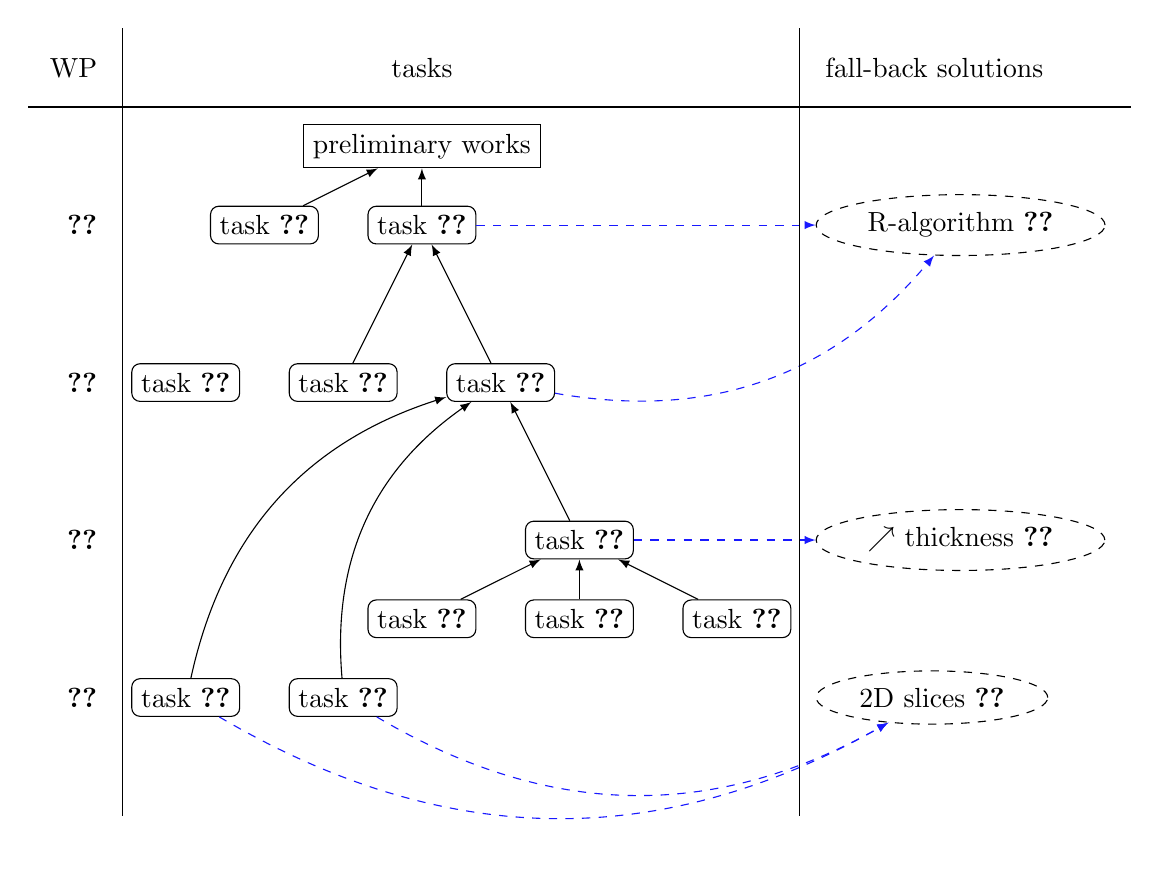
\begin{tikzpicture} 
\usetikzlibrary{shapes}

\tikzset{task/.style={draw,rectangle,rounded corners=3pt}}
\tikzset{sol/.style={draw,ellipse,dashed}}
\tikzset{toSol/.style={->,>=latex,dashed,color=blue!90!white}}
\tikzset{toTask/.style={->,>=latex}}

\node[left] at (0,8) {WP}; 
\node[left] at (0,6) {\ref{wp0}}; 
\node[left] at (0,4) {\ref{wp1}}; 
\node[left] at (0,2) {\ref{wp2}}; 
\node[left] at (0,0) {\ref{wp3}}; 

\node[right] at (9,8) {fall-back solutions};
\node[right,sol] (R) at (9,6) {R-algorithm \ref{riskppa}};
\node[right,sol] (C) at (9,2) { $\nearrow$ thickness \ref{riskestim}};
\node[right,sol] (S) at (9,0) {2D slices \ref{riskscale}};

\node at (4,8) {tasks};
\node[draw] (P) at (4,7) {preliminary works};

\node[task] (t0a) at (2,6) {task~\ref{task:reduction}};
\node[task] (t0b) at (4,6) {task~\ref{task:start}};
\draw[toTask] (t0a) -- (P);
\draw[toTask] (t0b) -- (P);
\draw[toSol] (t0b) -- (R);
\node[task] (t1a) at (1,4) {task~\ref{task:genmeth}};
\node[task] (t1b) at (3,4) {task~\ref{task:genexp}};
\node[task] (t1c) at (5,4) {task~\ref{task:genpat}};
\draw[toTask] (t1b) -- (t0b);
\draw[toTask] (t1c) -- (t0b);
\draw[toSol] (t1c) to[bend right] (R);
\node[task] (t2a) at (6,2) {task~\ref{task:normal}};
\node[task] (t2b) at (4,1) {task~\ref{task:conv}};
\node[task] (t2c) at (6,1) {task~\ref{task:approx}};
\node[task] (t2d) at (8,1) {task~\ref{task:rendering}};
\draw[toTask] (t2a) -- (t1c);
\draw[toSol] (t2a) -- (C);
\draw[toTask] (t2b) -- (t2a);
\draw[toTask] (t2c) -- (t2a);
\draw[toTask] (t2d) -- (t2a);
\node[task] (t3a) at (1,0) {task~\ref{task:global}};
\node[task] (t3b) at (3,0) {task~\ref{task:local}};
\draw[toTask] (t3a) to[bend left] (t1c);
\draw[toTask] (t3b) to[bend left] (t1c);
\draw[toSol] (t3a) to[bend right] (S);
\draw[toSol] (t3b) to[bend right] (S);

%\draw (-0.5,0) grid[step=1] (9,8);

\draw (-1,7.5) -- (13,7.5);
\draw (0.2,-1.5) -- (0.2,8.5);
\draw (8.8,-1.5) -- (8.8,8.5);

\end{tikzpicture}

  \caption{Dependency graph of the project tasks (see text for details).} %\sect{sec:schedule} for details.}
  \label{fig:tasks}
\end{figure}

One can clearly see in fig.~\ref{fig:tasks} that \ref{wp0} and \ref{wp1} can be started
at the beginning of the project, whereas \ref{wp2} and \ref{wp3}, which greatly depend
on tasks~\ref{task:start} and \ref{task:genpat}, respectively in \ref{wp0} and \ref{wp1},
must begin later. \ref{wp3} will start strictly after \ref{wp0} and \ref{wp1}, but \ref{wp2}
will start sooner, because we will first focus on convex parts and only task~\ref{task:start}
in \ref{wp0} is required for that.

To sum up, fig.~\ref{fig:gantt} shows the Gantt chart of the project schedule.
The WPs are listed on the vertical axis and time intervals on the horizontal axis.
The width of the horizontal dark blue bars show the duration of each WP. The first WP,
which mainly consists of short-term tasks is one-year long whereas the next ones are
two-year long. Deliverables are located at the finish date of each WP. They will be
provided in the form of technical reports at T+12 and T+30, and in the form of software
release at T+24 and T+48.

\begin{figure}[htbp]
  \centering
  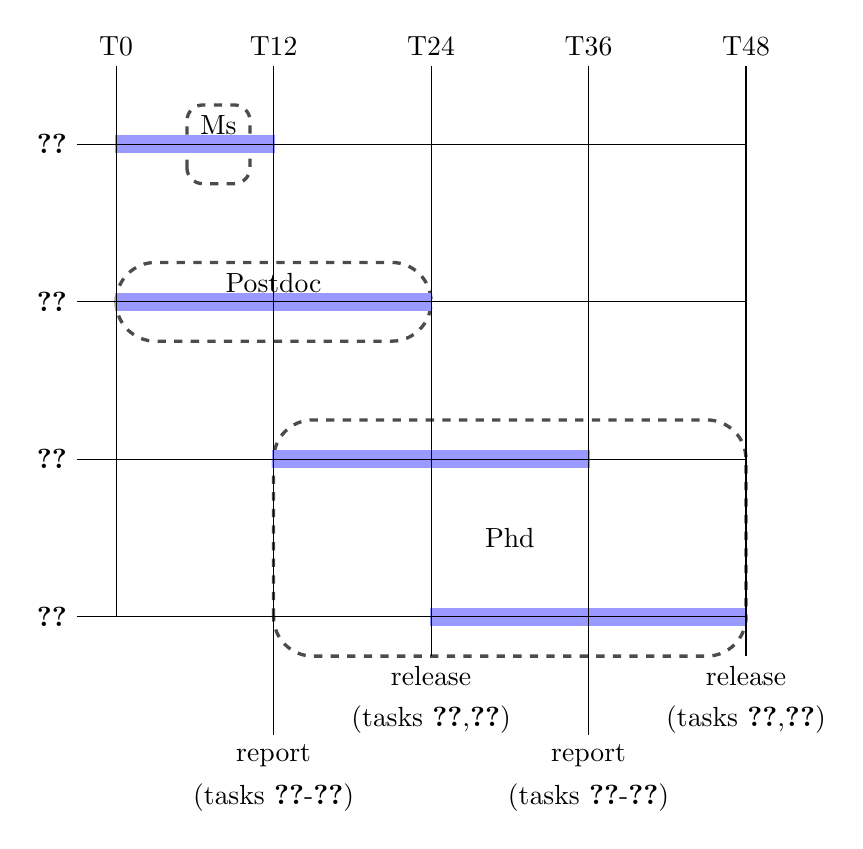
\begin{tikzpicture} 

\tikzset{%
  ebo unit/.store in=\ebounit,
  ebo corners/.style={rounded corners=#1\ebounit},
}

\node[above] at (0,7) {T0};
\node[above] at (2,7) {T12};
%\node[above] at (3,7) {T18};
\node[above] at (4,7) {T24};
\node[above] at (6,7) {T36};
\node[above] at (8,7) {T48};   

\node[left] at (-0.5,6) {\ref{wp0}}; 
\node[left] at (-0.5,4) {\ref{wp1}}; 
\node[left] at (-0.5,2) {\ref{wp2}}; 
\node[left] at (-0.5,0) {\ref{wp3}}; 

\tikzset{body/.style={very thick,dashed,color=black!70!white}}
\draw[draw,body,rounded corners=0.2cm] (0.9,5.5) rectangle (1.7,6.5) {};
\draw[draw,body,rounded corners=0.5cm] (0,3.5) rectangle (4,4.5) {};
\draw[draw,body,rounded corners=0.5cm] (2,-0.5) rectangle (8,2.5) {};

\tikzset{wp/.style={fill,thick,color=blue!40!white}}

\draw[draw,wp] (0,5.9) rectangle (2,6.1) {};
\draw[draw,wp] (0,3.9) rectangle (4,4.1) {};
\draw[draw,wp] (2,1.9) rectangle (6,2.1) {};
\draw[draw,wp] (4,-0.1) rectangle (8,0.1) {};

\node[above] at (1.3,6) {Ms};
\node[above] at (2,4) {Postdoc};
\node at (5,1) {Phd};

\draw (-0.5,0) grid[step=2] (8,7);

\tikzset{del/.style={fill}}

\draw[del] (4,-0.5) -- (4,7);
\node[below] at (4,-0.5) {release};
\node[below] at (4,-1) {(tasks~\ref{task:start},\ref{task:genpat})};
\draw[del] (8,-0.5) -- (8,7);
\node[below] at (8,-0.5) {release};
\node[below] at (8,-1) {(tasks~\ref{task:global},\ref{task:local})};

\draw[del] (2,-1.5) -- (2,7);
\node[below] at (2,-1.5) {report};
\node[below] at (2,-2) {(tasks~\ref{task:reduction}-\ref{task:genexp})};
\draw[del] (6,-1.5) -- (6,7);
\node[below] at (6,-1.5) {report};
\node[below] at (6,-2) {(tasks~\ref{task:normal}-\ref{task:rendering})};

\end{tikzpicture}

  \caption{Gantt chart for PARADIS' work packages. See \sect{sec:schedule} for details.}
  \label{fig:gantt}
\end{figure}

In addition, collaborators hired during the project and for which we request a financial support
are depicted with dashed grey rectangles.
The postdoctoral student (Postdoc) will be hired for working on \ref{wp1} at the beginning of the project.
The master student (MS) will work on \ref{wp0} during the first year and the PhD student (PhD) will be
hired after one year for working on \ref{wp2} and \ref{wp3}. If the master student demonstrate strong skills,
he will be an excellent applicant for the PhD grant.

\subsubsection{Requested means}
\label{sec:ressources}

\Comments{
Describe the means – those previously available and those requested - to achieve the objectives 
Scientific and technical justification of the requested means - per item of expenditure and by partner -, linked to the objectives of the proposal. Summarise the funding request in the table below in accordance with the information filled out on the website and with ANR’s grant allocation rules (règlement relatif aux modalités d’attribution des aides de l’ANR ).
Description of the context in terms of human and financial resources available thanks to previous or ongoing projects. }

\Comments{la demande en ressource devra être mieux justifiée (en particulier, l'apport plus concret d'un chercheur en postdoctorat (pas étudiant).}

The total required amount for PARADIS is about \textbf{260k \euro}, including management fees.
This section details our needs, which are summed up in table~\ref{tab:grant}.

\begin{table}[htbp]
  \caption{Requested means by item of expenditure}
  \centering
  \begin{tabular}{|l|r|}
    \hline 
    Expense                                      & Amount (in \euro) \\ \hline \hline
    Staff expenses                               & 205,212.00 \\ \hline
    Instruments and material costs               & 6,000.00  \\ \hline
%%    Building and ground costs                    & 0.00  \\ \hline
%%    Outsourcing / subcontracting                 & 0.00 \\ \hline
    Travel costs                                 & 30,200.00  \\  \hline
    SubTotal                                     & 241,412.00 \\ \hline \hline
    Administrative management \& structure costs & 19,296.96 \\ \hline \hline
    Requested                                    & 260,508.96 \\ \hline
    \hline
  \end{tabular}
  \label{tab:grant}
\end{table}

\textbf{Staff ($\approx$ 205k \euro).} As described in the scientific program (\sect{sec:wp} and \sect{sec:schedule}),
we request one PhD grant (3 years) and one master project funding (6 months).
We estimate this cost at  ($\approx$ 111k \euro). TODO detailler.
A same student would basically start working on \ref{wp0} during its master project and then
continue with \ref{wp2} and \ref{wp3} during its PhD thesis.
We also need a postdoctoral student for working on \ref{wp1} during two years ($\approx$ 95k \euro). 
The transdisciplinarity, difficulty and importance of \ref{wp1} requires an experienced student
that already has good technical abilities and an expert knowledge of at least digital geometry
or combinatorics on words. This position will let him gain new skills in a cutting-edge project
and launch its career. On the project side, this full-time worker will strengthen the synergy and
convergence of the team skills. 

\textbf{Travel costs ($\approx$ 30k \euro).}
We also request funds for one international travel (2,000 \euro~on average)
per year for the PI (4 years), the PhD student (3 years) and the postdoctoral student (2 years)
but only one during the whole project for the four other collaborators due to their lower involvement.
We estimate this cost at 2,000 x (4 years-PI + 3 years-PhD + 2 years-Postdoc + 4 collaborators) = 26,000 \euro. 

In addition, we would like to promote frequent face-to-face interactions between the team members.
We plan work meetings twice a year during two years with
S. Labb\'{e} \ref{wp0}\ref{wp1} (LABRI, Bordeaux) and
with B. Kerautret \ref{wp3} (LORIA, Nancy),
but during four years
with J-O. Lachaud \ref{wp0}\ref{wp2}\ref{wp3} (LAMA, Chamb\'{e}ry).
We estimate the cost of a work meeting at 275 \euro~per person
for Lyon-Bordeaux and for Lyon-Nancy,
but only 60 \euro~for Lyon-Chamb\'{e}ry.
With three travelers on average per work meeting, we estimate the total cost at:

\begin{tabular}{lrr}
  (Lyon-Bordeaux) & 275 x 2 years x 3 travelers on average =& 1,650 \euro~\\ 
  (Lyon-Nancy) & 275 x 2 years x 3 travelers on average =& 1,650 \euro~\\
  (Lyon-Chamb\'{e}ry) & 60 x 4 years x 3 travelers on average =& 720 \euro~\\
  Total & ~ & 4,200 \euro~\\
\end{tabular}
%% \begin{itemize}
%%   \item [~]  = 1,650 \euro~ 
%%   \item [$+$] 275 x 2 years x 3 travelers on average = 1,650 \euro
%%   \item [$+$] 60 x 4 years x 3 travelers on average = 720 \euro
%%   \item [$=$] 4,200 \euro. 
%% \end{itemize}

\textbf{Material costs ($\approx$ 6k \euro).}
We request four standard computers (1500 \euro) for the PI and each student to work on.
We estimate this cost at 1,500 \euro~x 4 = 6000 \euro. 
